\documentclass{article}
\usepackage[utf8]{inputenc}
\usepackage{cancel}
\usepackage{amssymb}
\usepackage{graphicx}
\graphicspath{{Images/}}
\usepackage{chngcntr}
\counterwithin{equation}{section}


\title{Project 1 (Astrophysics)}
\author{Michael Nameika}
\date{January 2022}

\begin{document}

\maketitle
Useful formulas:
\begin{equation}
    A_{triangle} = \frac{1}{2}(b)(h)
\end{equation}
\begin{equation}
    A_{sector} = \frac{\theta}{2\pi}(\pi R^2)
\end{equation}
\begin{equation}
    V = \frac{d}{t}
\end{equation}

\section{}
\begin{center}
    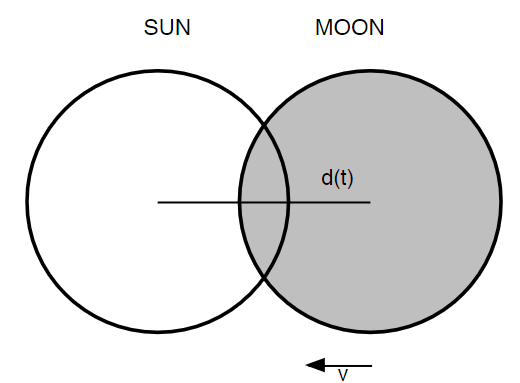
\includegraphics[scale = 0.8]{eclipsepic.PNG}
    \newline\newline
    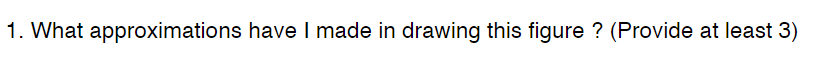
\includegraphics[scale = 0.8]{projectq1.PNG}
\end{center}

Approximations:
\begin{itemize}
    \item The Sun and Moon are assumed to be the same angular size
    \item It is assumed that after some time, the center point of the Sun and Moon will share the same point in space.
    \item The Sun is assumed to be stationary in the sky
\end{itemize}
\section{}
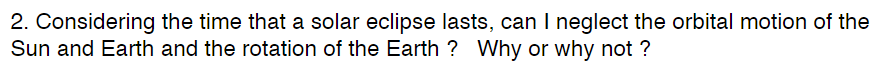
\includegraphics[scale = 0.8]{projectq2.PNG}
Well, a solar eclipse typically lasts only a few minutes, and since the orbit of the Earth around the Sun takes an entire year ($\approx 5.260\times10^5 \:minutes$). There are about $5$ orders of magnitude difference between the time in minutes for a solar eclipse and an Earth orbit. Now, a sidereal day contains approximately $1436$ minutes, which is $3$ orders of magnitude greater than the time of a solar eclipse. So, I would say that is fine to neglect the rotation of the Earth and its orbit.


\section{}
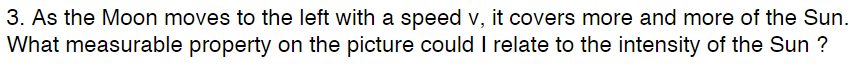
\includegraphics[scale = 0.8]{projectq3.PNG}
The angle $\theta$, the distance between the midpoints of the Sun and Moon, and the eclipsed area.

\section{}
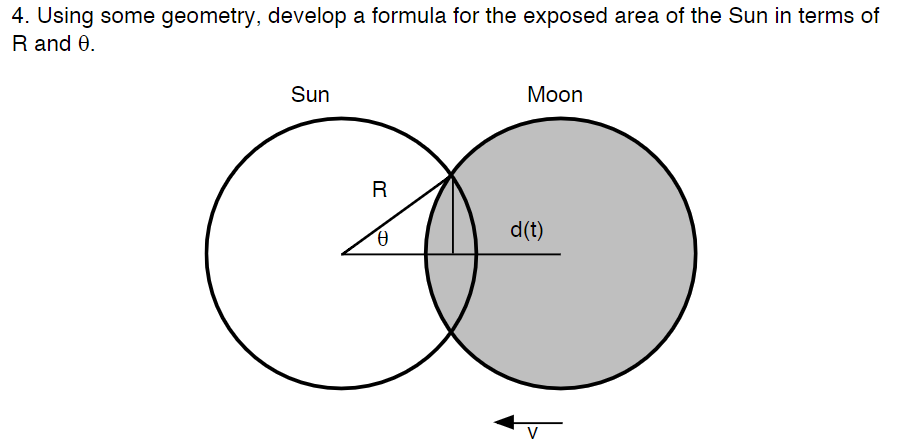
\includegraphics[scale = 0.8]{projectq4.PNG}
Notice from the picture that if we find the area of the sector subtended by $\theta$, and subtract the area of the right triangle formed with $R$, $\theta$, and the distance between the midpoints, we will get $\frac{1}{4}$ of the area of the shaded region.
\newline
Using the sector area formula (0.2), we will find the following:
\begin{center}
    $A_{sector} = \frac{\cancel{\pi} R^2}{2\cancel{\pi}}\theta$
\end{center}
\begin{equation}
    = \frac{R^2}{2}\theta
\end{equation}

And the area of the triangle by (0.1):
\begin{center}
    $A_{triangle} = \frac{1}{2}*R\cos{(\theta)}*R\sin{(\theta)}\footnote{Notice the base is given by cos($\theta$) and the height is given by sin($\theta$).}$
\end{center}
\begin{center}
    $= \frac{R^2}{2}\sin{(\theta)}\cos{(\theta)}$
\end{center}
\begin{equation}
    = \frac{R^2}{4}\sin{(2\theta)}
\end{equation}
Now, subtracting (4.2) from (4.1), and multiply the result by $4$, we will get the area of the eclipsed region:
\begin{center}
    $A_{eclipsed\:region} = 4(\frac{R^2}{2}\theta - \frac{R^2}{4}\sin{(2\theta)})$
\end{center}
\begin{equation}
    = 2R^2\theta - R^2\sin{(2\theta)}
\end{equation}
Now, to find the area of the non-shaded region, let us subtract (4.3) from the area of the Sun's disc:
\begin{center}
    $A_{nonshaded\:region} = \pi R^2 - (2R^2\theta - R^2\sin{(2\theta)})$
\end{center}
\begin{equation}
    = R^2(\pi - 2\theta + \sin{(2\theta)})
\end{equation}
So the area of the exposed region in terms of $R$ and $\theta$ is given by (4.4).

\section{}
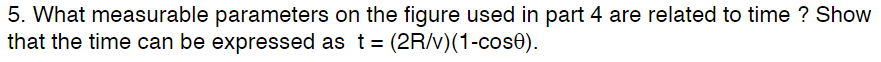
\includegraphics[scale = 0.8]{projectq5.PNG}
From equation (0.3), we can see that 
\begin{equation}
    d(t) = Vt
\end{equation}

Knowing that $d$ is the distance from the center of the Sun's disc to the Moon's disc, notice from $4$ and equation (4.2), we have that the distance $d$ is going to be 
\begin{equation}
    d = 2R\cos{(\theta)}
\end{equation}
But also notice that when $\theta = 0$, $t = 0$ (The eclipse has just begun). So we can claim (without proof) that $t$ is related to (5.2) by 
\begin{equation}
    2R(1-\cos{(\theta))}
\end{equation}
Now we have two expressions for $d$, so let's set them equal to each other:
\begin{center}
    $Vt = 2R(1-\cos{(\theta)})$
\end{center}
\begin{equation}
    t = \frac{2R}{V}(1-\cos{(\theta)})
\end{equation}
The desired result.
\begin{flushright}
    $\square$
\end{flushright}
\section{}
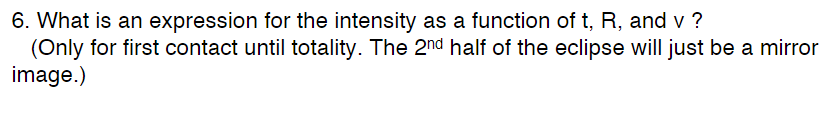
\includegraphics[scale = 0.8]{projectq6.PNG}
We wish to find an expression for the intensity as a function of $t$, $R$ and $V$. From equation (5.4), we can solve for $\theta$ and get it in terms of $t$, $R$, and $V$. With a little algebra, we get
\[\theta = \cos^{-1}{(1-\frac{Vt}{2R})}\]
Now, using that the Sun's intensity is proportional to the exposed area,
\[I \propto A\]
\[ A =  R^2(\pi - 2\cos^{-1}{(1-\frac{Vt}{2R})} + \sin{(2\cos^{-1}{(1-\frac{Vt}{2R})})})\]
Let $k$ be a constant of proportionality. Then we have
\begin{equation}
    I = kR^2(\pi - 2\cos^{-1}{(1-\frac{Vt}{2R})} + \sin{(2\cos^{-1}{(1-\frac{Vt}{2R})})})
\end{equation}

\section{}
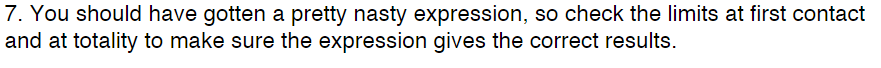
\includegraphics[scale = 0.8]{projectq7.PNG}
At first contactc ($t=0$), the disc of the Sun and the Moon will be tangent, so the total eclipsed area will be $0$. We should expect the intensity of the Sun to be exactly proportional to the full area of the Sun. That is, 
\[I \propto k\pi R^2\]
Plugging in $t=0$ into (6.1), we get the following:
\[I = kR^2(\pi - 2\cos^{-1}{(1-\frac{V*0}{2R})} + \sin{(2\cos^{-1}{(1-\frac{V*0}{2R})})})\]
\[ = kR^2(\pi -2\cos^{-1}{(1-0)} + \sin{(2\cos^{-1}{(1-0)})})\]
\[ = kR^2(\pi - 2(0) + \sin{(2(0))}\]
\[ = k\pi R^2\]
Thus, at $t = 0$, intensity is proportional to the full area, which is what we hoped to get. Now let's check the limit at the full eclipse. That is, $A = 0$. First, let's solve for t. We know that the full eclipse will occur when $\theta = \frac{\pi}{2}$. Then using equation (5.4), we can see that the total eclipse occurs when 
\[t = \frac{2R}{V}\]
Plugging this into (6.1), we will get
\[I = kR^2(\pi - 2\cos^{-1}{(1 - \frac{\cancel{V}*\frac{\cancel{2R}}{\cancel{V}}}{\cancel{2R}})} + \sin{(2\cos^{-1}{(1 - \frac{\cancel{V}*\frac{\cancel{2R}}{\cancel{V}}}{\cancel{2R}})})})\]
\[ = kR^2(\pi - 2\cos^{-1}{(0)} + \sin{(2*0)})\]
\[ = kR^2(\pi - 2\frac{\pi}{2} + 0)\]
\[ = kR^2(\pi - \pi)\]
\[ = kR^2(0)\]
\[ = 0\]
Thus, at the moment of the total eclipse, the total intensity of the Sun will be $0$, which is what we expected.
\begin{flushright}
    $\square$
\end{flushright}
\section{}
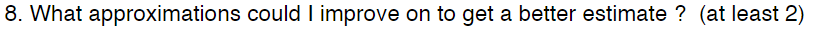
\includegraphics[scale = 0.8]{projectq8.PNG}
\begin{itemize}
    \item Use that the Sun is not stationary in the sky (That is, take into account Earth's rotation).
    \item Could use that the angular size of the Moon is different from the Sun (for example, if we expect an annular eclipse, we could reduce the angular size of the Moon a little bit, or for a total eclipse, we could increase the Moon's angular size).
\end{itemize}




\end{document}